\documentclass[border=18pt,tikz]{standalone}
\usepackage{amsmath,amssymb,bm}
\usetikzlibrary{arrows.meta,positioning,calc,decorations.pathreplacing,fit,backgrounds}

% ============================================================
%  arch_common.tex  --  shared TikZ styles for MTP-PINN figures
%  All fonts bumped to \large; inner sep generous; no overlaps.
% ============================================================
\newcommand{\ArchBlockFont}{\large}
\newcommand{\ArchPhaseHdr}{\large\bfseries\color{black!80}}

%% --- Colour palette --------------------------------------------------------
\definecolor{KinFill}{RGB}{224,247,250}
\definecolor{KinDraw}{RGB}{0,131,143}
\definecolor{PhyFill}{RGB}{255,243,224}
\definecolor{PhyDraw}{RGB}{230,81,0}
\definecolor{NrmFill}{RGB}{243,229,245}
\definecolor{NrmDraw}{RGB}{106,27,154}
\definecolor{CatFill}{RGB}{255,249,196}
\definecolor{CatDraw}{RGB}{245,127,23}
\definecolor{MlpFill}{RGB}{227,242,253}
\definecolor{MlpDraw}{RGB}{21,101,192}
\definecolor{TanhFill}{RGB}{237,231,246}
\definecolor{TanhDraw}{RGB}{123,31,162}
\definecolor{AddFill}{RGB}{241,248,233}
\definecolor{AddDraw}{RGB}{85,139,47}
\definecolor{OutFill}{RGB}{232,245,233}
\definecolor{OutDraw}{RGB}{46,125,50}
\definecolor{LossFill}{RGB}{255,235,238}
\definecolor{LossDraw}{RGB}{183,28,28}
\definecolor{PhysBpFill}{RGB}{255,248,225}
\definecolor{PhysBpDraw}{RGB}{249,168,37}
\definecolor{NoteFill}{RGB}{245,245,245}
\definecolor{NoteDraw}{RGB}{100,100,100}

%% --- TikZ styles -----------------------------------------------------------
\tikzset{
  every node/.style={align=center},
  line cap=round,
  %% base block
  blk/.style={
    draw=gray!55,
    line width=1.6pt,
    rounded corners=6pt,
    inner sep=14pt,
  },
  %% domain blocks
  kinBlk/.style={
    blk, fill=KinFill, draw=KinDraw,
    minimum width=4.2cm,
    font=\ArchBlockFont,
  },
  phyBlk/.style={
    blk, fill=PhyFill, draw=PhyDraw,
    minimum width=5.8cm,
    font=\ArchBlockFont,
  },
  nrmBlk/.style={
    blk, fill=NrmFill, draw=NrmDraw,
    minimum width=4.0cm,
    font=\ArchBlockFont,
  },
  catBlk/.style={
    blk, fill=CatFill, draw=CatDraw,
    minimum width=2.2cm,
    font=\ArchBlockFont,
  },
  mlpBlk/.style={
    blk, fill=MlpFill, draw=MlpDraw,
    minimum width=3.6cm,
    font=\ArchBlockFont,
  },
  fcBlk/.style={
    blk, fill=MlpFill, draw=MlpDraw,
    minimum width=3.4cm,
    font=\ArchBlockFont,
  },
  tanhBlk/.style={
    blk, fill=TanhFill, draw=TanhDraw,
    minimum width=3.4cm,
    font=\ArchBlockFont,
  },
  outBlk/.style={
    blk, fill=OutFill, draw=OutDraw,
    minimum width=3.4cm,
    font=\ArchBlockFont,
  },
  addBlk/.style={
    circle,
    draw=AddDraw,
    fill=AddFill,
    line width=1.5pt,
    minimum size=1.4cm,
    font=\LARGE\bfseries,
  },
  gtBlk/.style={
    blk, draw=NoteDraw, fill=NoteFill,
    line width=1.2pt,
    rounded corners=5pt,
    inner sep=12pt,
    font=\ArchBlockFont,
    minimum width=3.2cm,
  },
  lossBlk/.style={
    blk, fill=LossFill, draw=LossDraw,
    line width=1.4pt,
    inner sep=16pt,
    font=\ArchBlockFont,
  },
  bpBlk/.style={
    blk, fill=PhysBpFill, draw=PhysBpDraw,
    inner sep=10pt,
    font=\ArchBlockFont,
  },
  %% arrows
  arr/.style={
    -{Stealth[length=11pt,width=9pt]},
    line width=1.8pt,
    black!80,
  },
  darr/.style={
    -{Stealth[length=9pt,width=7.5pt]},
    line width=1.5pt,
    dashed,
    dash pattern=on 5pt off 3pt,
    black!50,
  },
  bparr/.style={
    -{Stealth[length=11pt,width=9pt]},
    line width=1.8pt,
    PhyDraw!90,
    rounded corners=4pt,
  },
  %% edge labels
  dim/.style={
    font=\large,
    fill=white,
    inner sep=3pt,
    above=1pt,
    midway,
    sloped=false,
  },
  diml/.style={
    font=\large,
    fill=white,
    inner sep=3pt,
    below=1pt,
    midway,
  },
  phaseHdr/.style={
    font=\ArchPhaseHdr,
    inner sep=0pt,
    outer sep=0pt,
    anchor=south west,
  },
}


\def\BH{5.2cm}
\def\IH{2.3cm}

\begin{document}
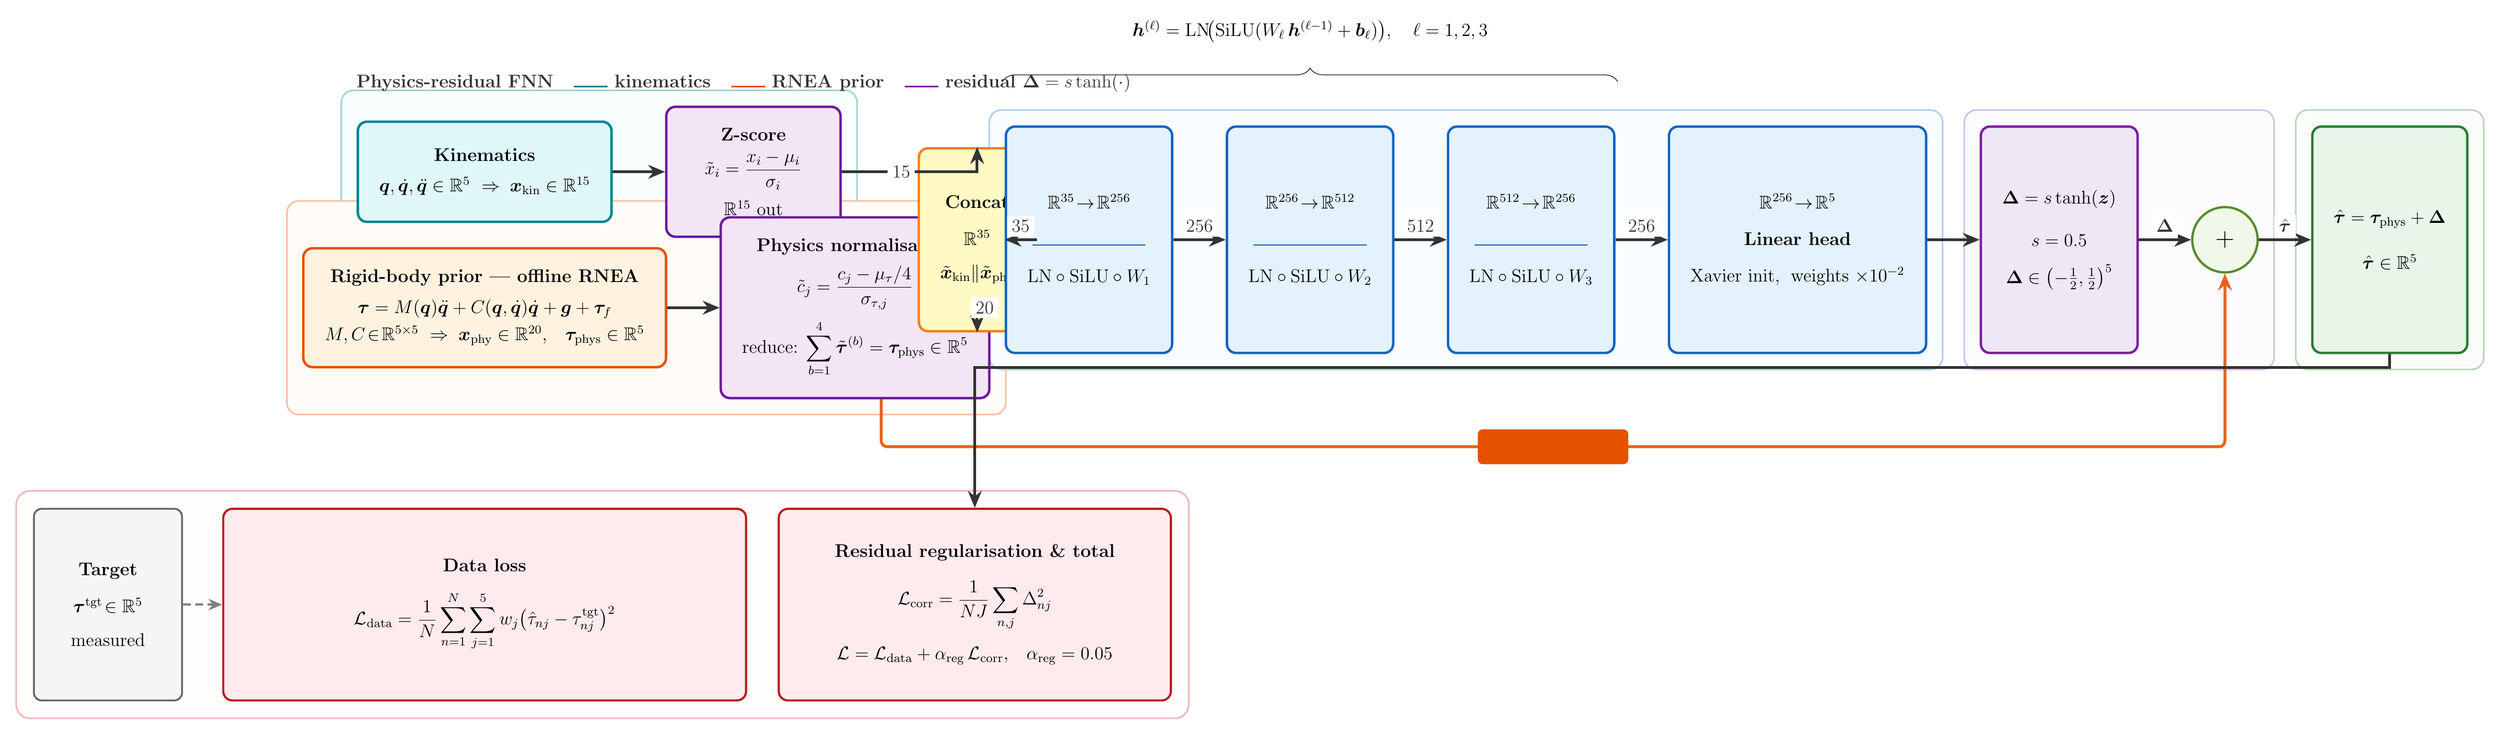
\begin{tikzpicture}[node distance=1.2cm]

%%═══════════════════════════════ INPUT COLUMN ════════════════════════════════
\node[kinBlk,
      minimum height=\IH, minimum width=4.4cm]
  (KINPUT) at (0,0) {%
  \textbf{Kinematics}\\[6pt]
  $\bm{q},\dot{\bm{q}},\ddot{\bm{q}}\in\mathbb{R}^{5}$
  $\;\Rightarrow\;\bm{x}_{\mathrm{kin}}\in\mathbb{R}^{15}$
};

\node[phyBlk,
      minimum height=\IH, minimum width=5.8cm,
      below=0.55cm of KINPUT.south, anchor=north]
  (PINPUT) {%
  \textbf{Rigid-body prior — offline RNEA}\\[6pt]
  $\bm{\tau}=M(\bm{q})\ddot{\bm{q}}+C(\bm{q},\dot{\bm{q}})\dot{\bm{q}}+\bm{g}+\bm{\tau}_{f}$\\[4pt]
  {\large $M,C\!\in\!\mathbb{R}^{5\times 5}$
    $\;\Rightarrow\;\bm{x}_{\mathrm{phy}}\in\mathbb{R}^{20}$,\quad
    $\bm{\tau}_{\mathrm{phys}}\in\mathbb{R}^{5}$}
};

%%═══════════════════════════════ NORM COLUMN ═════════════════════════════════
\node[nrmBlk,
      minimum height=\IH, minimum width=4.0cm,
      right=1.2cm of KINPUT]
  (KNORM) {%
  \textbf{Z-score}\\[6pt]
  $\tilde{x}_{i}=\dfrac{x_{i}-\mu_{i}}{\sigma_{i}}$\\[6pt]
  $\mathbb{R}^{15}$ out
};

\node[nrmBlk,
      minimum height=\IH, minimum width=4.8cm,
      right=1.2cm of PINPUT.east, anchor=west]
  (PNORM) {%
  \textbf{Physics normalisation}\\[6pt]
  $\tilde{c}_{j}=\dfrac{c_{j}-\mu_{\tau}/4}{\sigma_{\tau,j}}$\\[6pt]
  {\large reduce:
    $\displaystyle\sum_{b=1}^{4}\tilde{\bm{\tau}}^{(b)}=\bm{\tau}_{\mathrm{phys}}\in\mathbb{R}^{5}$}
};

%%═══════════════════════════════ CONCAT ══════════════════════════════════════
\coordinate (CatX) at ($(KNORM.east)!0.5!(PNORM.east) + (1.4cm,0)$);
\node[catBlk,
      minimum width=2.4cm, minimum height=4.2cm]
  (CAT) at (CatX) {%
  \textbf{Concat}\\[10pt]
  $\mathbb{R}^{35}$\\[8pt]
  {\large $\tilde{\bm{x}}_{\mathrm{kin}}\Vert\tilde{\bm{x}}_{\mathrm{phy}}$}
};

%%═══════════════════════════════ MLP TRUNK ═══════════════════════════════════
\node[mlpBlk, minimum height=\BH, minimum width=3.6cm,
      right=1.2cm of CAT, anchor=center]
  (H1) {%
  $\mathbb{R}^{35}\!\to\!\mathbb{R}^{256}$\\[10pt]
  \textcolor{MlpDraw}{\rule{2.6cm}{0.9pt}}\\[10pt]
  $\mathrm{LN}\circ\mathrm{SiLU}\circ W_{1}$
};

\node[mlpBlk, minimum height=\BH, minimum width=3.6cm,
      right=1.2cm of H1]
  (H2) {%
  $\mathbb{R}^{256}\!\to\!\mathbb{R}^{512}$\\[10pt]
  \textcolor{MlpDraw}{\rule{2.6cm}{0.9pt}}\\[10pt]
  $\mathrm{LN}\circ\mathrm{SiLU}\circ W_{2}$
};

\node[mlpBlk, minimum height=\BH, minimum width=3.6cm,
      right=1.2cm of H2]
  (H3) {%
  $\mathbb{R}^{512}\!\to\!\mathbb{R}^{256}$\\[10pt]
  \textcolor{MlpDraw}{\rule{2.6cm}{0.9pt}}\\[10pt]
  $\mathrm{LN}\circ\mathrm{SiLU}\circ W_{3}$
};

\node[fcBlk, minimum height=\BH, minimum width=3.4cm,
      right=1.2cm of H3]
  (FC) {%
  $\mathbb{R}^{256}\!\to\!\mathbb{R}^{5}$\\[10pt]
  \textbf{Linear head}\\[10pt]
  {\large Xavier init,\; weights $\times 10^{-2}$}
};

\node[tanhBlk, minimum height=\BH, minimum width=3.4cm,
      right=1.2cm of FC]
  (TANH) {%
  $\bm{\Delta}=s\tanh(\bm{z})$\\[14pt]
  $s=0.5$\\[10pt]
  $\bm{\Delta}\in\bigl(-\tfrac{1}{2},\tfrac{1}{2}\bigr)^{5}$
};

\node[addBlk, minimum size=1.5cm, right=1.2cm of TANH]
  (ADD) {$+$};

\node[outBlk, minimum height=\BH, minimum width=3.4cm,
      right=1.2cm of ADD]
  (OUT) {%
  $\hat{\bm{\tau}}=\bm{\tau}_{\mathrm{phys}}+\bm{\Delta}$\\[16pt]
  $\hat{\bm{\tau}}\in\mathbb{R}^{5}$
};

%%═══════════════════════════════ ARROWS ═════════════════════════════════════
\draw[arr](KINPUT.east) -- (KNORM.west);
\draw[arr](PINPUT.east) -- (PNORM.west);

\draw[arr](KNORM.east) -| node[pos=0.22,font=\large,fill=white,inner sep=3pt]{15} (CAT.north);
\draw[arr](PNORM.east) -| node[pos=0.22,font=\large,fill=white,inner sep=3pt]{20} (CAT.south);

\draw[arr](CAT) -- node[dim]{35}  (H1);
\draw[arr](H1)  -- node[dim]{256} (H2);
\draw[arr](H2)  -- node[dim]{512} (H3);
\draw[arr](H3)  -- node[dim]{256} (FC);
\draw[arr](FC)  -- (TANH);
\draw[arr](TANH)-- node[dim]{$\bm{\Delta}$} (ADD);
\draw[arr](ADD) -- node[dim]{$\hat{\bm{\tau}}$} (OUT);

%%── Physics shortcut: route BELOW the full row, emerge at ADD.south ──────────
\coordinate (PShortStart) at ($(PNORM.south)+(0.6,0)$);
%% lane sits 1.8cm below the bottom of the input blocks
\coordinate (LaneY) at ($(PINPUT.south)+(0,-1.8cm)$);
\coordinate (PtA) at (PShortStart |- LaneY);          % go straight down
\coordinate (PtB) at (ADD.south |- LaneY);              % run right at lane level
\draw[bparr, line width=1.9pt]
  (PShortStart) -- (PtA) -- (PtB) -- (ADD.south);
\node[fill=white, draw=PhyDraw, rounded corners=3pt,
      inner sep=5pt, font=\large\bfseries, color=PhyDraw]
  at ($(PtA)!0.5!(PtB)$) {$\bm{\tau}_{\mathrm{phys}}$ (shortcut)};

%%═══════════════════════════════ BRACE ══════════════════════════════════════
\coordinate (BL) at ([yshift=1.0cm,xshift=-0.05cm]H1.north west);
\coordinate (BR) at ([yshift=1.0cm,xshift= 0.05cm]H3.north east);
\draw[decorate,decoration={brace,amplitude=9pt}]
  (BL)--(BR)
  node[midway,above=22pt,font=\large\itshape]{%
    $\bm{h}^{(\ell)}=\mathrm{LN}\!\bigl(\mathrm{SiLU}(W_\ell\,\bm{h}^{(\ell-1)}+\bm{b}_\ell)\bigr),\quad\ell=1,2,3$};

%%═══════════════════════════════ BACKGROUND FILLS ═══════════════════════════
\begin{scope}[on background layer]
  \node[fit=(KINPUT)(KNORM), inner sep=10pt,
        draw=KinDraw!35,fill=KinFill!22,
        rounded corners=8pt,line width=1.1pt]{};
  \node[fit=(PINPUT)(PNORM), inner sep=10pt,
        draw=PhyDraw!35,fill=PhyFill!22,
        rounded corners=8pt,line width=1.1pt]{};
  \node[fit=(H1)(H2)(H3)(FC), inner sep=10pt,
        draw=MlpDraw!32,fill=MlpFill!18,
        rounded corners=8pt,line width=1.1pt]{};
  \node[fit=(TANH)(ADD), inner sep=10pt,
        draw=TanhDraw!30,fill=TanhFill!18,
        rounded corners=8pt,line width=1.0pt]{};
  \node[fit=(OUT), inner sep=10pt,
        draw=OutDraw!32,fill=OutFill!18,
        rounded corners=8pt,line width=1.1pt]{};
\end{scope}

%%═══════════════════════════════ LOSS BAND ═══════════════════════════════════
%% Anchor below the physics-shortcut lane
\coordinate (LossTop) at ($(LaneY)+(0,-1.4cm)$);

\node[lossBlk, anchor=north, minimum height=4.4cm, minimum width=12.0cm]
  (LOSSD) at (LossTop) {%
  \textbf{Data loss}\\[12pt]
  $\displaystyle
    \mathcal{L}_{\mathrm{data}}
    =\frac{1}{N}\sum_{n=1}^{N}\sum_{j=1}^{5}
     w_{j}\bigl(\hat{\tau}_{nj}-\tau^{\mathrm{tgt}}_{nj}\bigr)^{2}$
};

\node[lossBlk, anchor=north west, minimum height=4.4cm, minimum width=9.0cm]
  (LOSSR) at ($(LOSSD.north east)+(0.7,0)$) {%
  \textbf{Residual regularisation \& total}\\[12pt]
  $\displaystyle
    \mathcal{L}_{\mathrm{corr}}
    =\frac{1}{NJ}\sum_{n,j}\Delta_{nj}^{2}$\\[10pt]
  $\mathcal{L}=\mathcal{L}_{\mathrm{data}}+\alpha_{\mathrm{reg}}\,\mathcal{L}_{\mathrm{corr}}$,\quad
  $\alpha_{\mathrm{reg}}=0.05$
};

\node[gtBlk, anchor=east, minimum height=4.4cm, minimum width=3.4cm]
  (GT) at ($(LOSSD.west)-(0.9,0)$) {%
  \textbf{Target}\\[10pt]
  $\bm{\tau}^{\mathrm{tgt}}\!\in\mathbb{R}^{5}$\\[8pt]
  {\large measured}
};

\draw[arr](OUT.south) -- ++(0,-0.3) -| (LOSSR.north);
\draw[darr](GT.east) -- (LOSSD.west);

\begin{scope}[on background layer]
  \node[fit=(GT)(LOSSD)(LOSSR), inner sep=11pt,
        draw=LossDraw!30,fill=LossFill!15,
        rounded corners=9pt,line width=1.1pt]{};
\end{scope}

%%═══════════════════════════════ TITLE ═══════════════════════════════════════
\node[phaseHdr] at ($(KINPUT.north west)+(0,0.65cm)$){%
  \textbf{Physics-residual FNN}\quad
  \textcolor{KinDraw}{\rule{22pt}{1.3pt}}~kinematics\quad
  \textcolor{PhyDraw}{\rule{22pt}{1.3pt}}~RNEA prior\quad
  \textcolor{TanhDraw}{\rule{22pt}{1.3pt}}~residual $\bm{\Delta}=s\tanh(\cdot)$
};

\end{tikzpicture}
\end{document}


\begin{document}
%% scale=1.12 keeps labels readable without shrinking relative to page margins
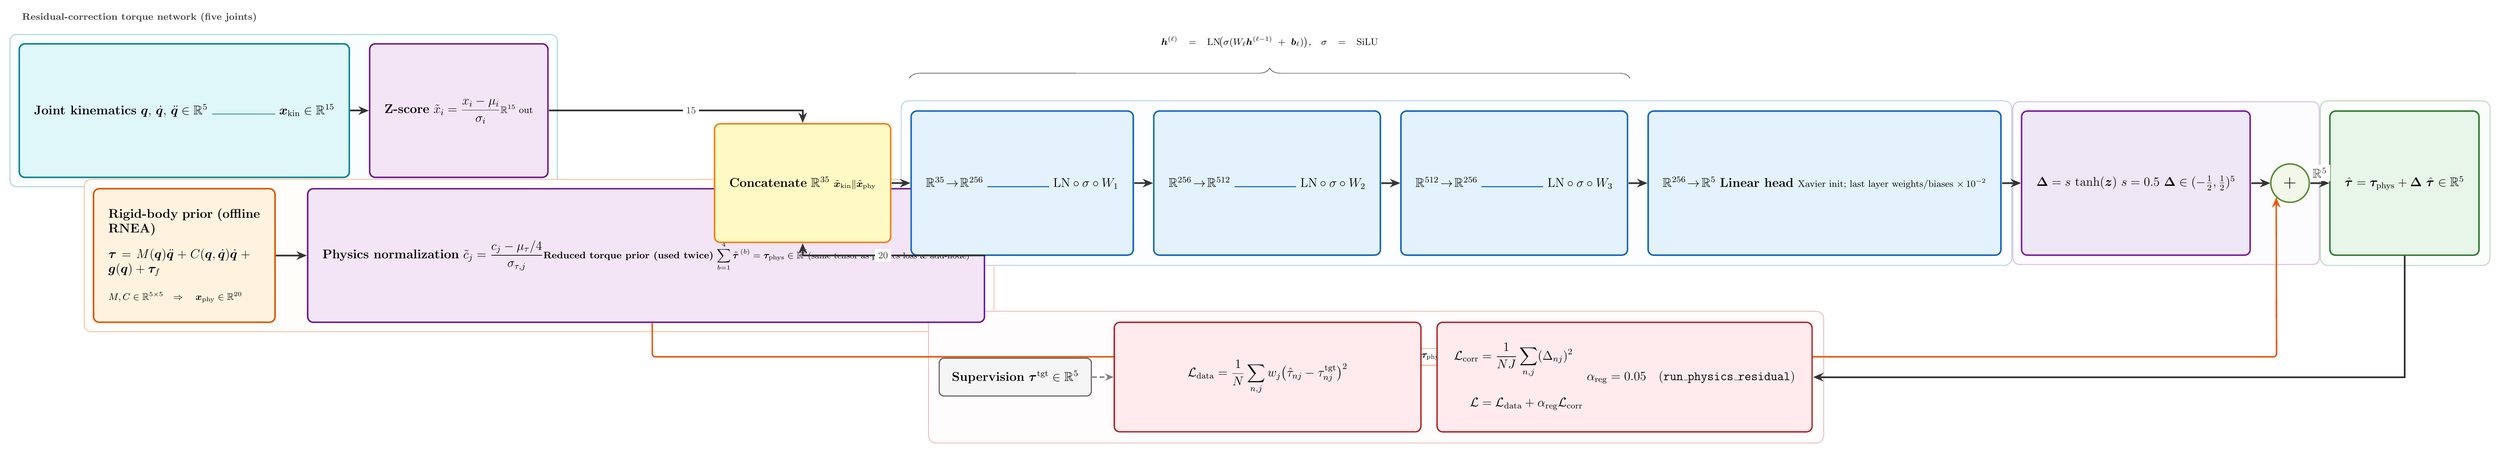
\begin{tikzpicture}[
    scale=1.12,
    every node/.style={transform shape},
    node distance=0.62cm,
  ]

\newcommand{\RailH}{4.45cm}% vertical extent of kinematics / physics columns
\newcommand{\FwdH}{4.8cm}% MLP row (slightly taller for legibility)

%% ========= row 1--2 : dual inputs ============================================
\node[kinBlk, minimum height=\RailH, minimum width=3.35cm](KINPUT) at (0,0){%
    \textbf{Joint kinematics}\\[9pt]
    $\bm{q},\,\dot{\bm{q}},\,\ddot{\bm{q}}\in\mathbb{R}^5$\\[8pt]
    \textcolor{KinDraw}{\rule{2.1cm}{0.82pt}}\\[8pt]
    $\bm{x}_{\mathrm{kin}}\in\mathbb{R}^{15}$%
};

\node[phyBlk, minimum height=\RailH,
      text width=5.05cm,
      align=left,below=0.32cm of KINPUT.south,anchor=north](PINPUT){%
    \textbf{Rigid-body prior (offline RNEA)}\\[10pt]
    $\displaystyle
      \bm{\tau}=M(\bm{q})\ddot{\bm{q}}
      +C(\bm{q},\dot{\bm{q}})\dot{\bm{q}}
      +\bm{g}(\bm{q})+\bm{\tau}_f$
    \\[12pt]{\small $M,C\in\mathbb{R}^{5{\times}5}$\quad
    $\Rightarrow\quad\bm{x}_{\mathrm{phy}}\in\mathbb{R}^{20}$}%
};

\node[nrmBlk,minimum height=\RailH,minimum width=3.15cm,right=of KINPUT](KNORM){%
    \textbf{Z-score}\\[12pt]
    $\displaystyle\tilde{x}_i=\frac{x_i-\mu_i}{\sigma_i}$\\[16pt]{\small$\mathbb{R}^{15}$ out}%
};

\node[nrmBlk,
     minimum height=\RailH,
     minimum width=3.45cm,
     right=1.03cm of PINPUT.east,anchor=west](PNORM){%
    \textbf{Physics normalization}\\[12pt]
    $\displaystyle\tilde{c}_j=\frac{c_j-\mu_\tau/4}{\sigma_{\tau,j}}$
    \\[16pt]{\small\textbf{Reduced torque prior (used twice)}\\[11pt]
    $\displaystyle\sum_{b=1}^{4}\tilde{\bm{\tau}}^{\,(b)}
     = \bm{\tau}_{\mathrm{phys}}\in\mathbb{R}^5$%
    \\
    {\footnotesize (same tensor as physics loss \& add-node)}}%
};

%% Concatenate (wider footprint — avoids crowding PNORM arrows)
\node[
  catBlk,
  minimum width=1.92cm,
  minimum height=3.95cm,
  at={($(KNORM.east)!0.5!(PNORM.east)+(1.18cm,0)$)}
](CAT){%
  \textbf{Concatenate}\\[12pt]
  $\mathbb{R}^{35}$\\[10pt]
  {\small $\tilde{\bm{x}}_{\mathrm{kin}}\Vert\tilde{\bm{x}}_{\mathrm{phy}}$}%
};

%% ========= MLP trunk ==========================================================
\node[mlpBlk,minimum height=\FwdH,minimum width=2.96cm,right=of CAT](H1){%
    $\mathbb{R}^{35}\!\to\!\mathbb{R}^{256}$\\[12pt]
    \textcolor{MlpDraw}{\rule{2.05cm}{0.78pt}}\\[12pt]
    $\mathrm{LN}\circ\sigma\circ W_1$%
};

\node[mlpBlk,minimum height=\FwdH,minimum width=2.96cm,right=of H1](H2){%
    $\mathbb{R}^{256}\!\to\!\mathbb{R}^{512}$\\[12pt]
    \textcolor{MlpDraw}{\rule{2.05cm}{0.78pt}}\\[12pt]
    $\mathrm{LN}\circ\sigma\circ W_2$%
};

\node[mlpBlk,minimum height=\FwdH,minimum width=2.96cm,right=of H2](H3){%
    $\mathbb{R}^{512}\!\to\!\mathbb{R}^{256}$\\[12pt]
    \textcolor{MlpDraw}{\rule{2.05cm}{0.78pt}}\\[12pt]
    $\mathrm{LN}\circ\sigma\circ W_3$%
};

\node[fcBlk,minimum height=\FwdH,minimum width=2.89cm,right=of H3](FCOUT){%
    $\mathbb{R}^{256}\!\to\!\mathbb{R}^{5}$\\[16pt]
    \textbf{Linear head}\\[12pt]
    {\small Xavier init; last layer weights/biases $\times\,10^{-2}$}%
};

\node[tanhBlk,minimum height=\FwdH,minimum width=2.85cm,right=of FCOUT](TANH){%
    $\bm{\Delta}=s\,\tanh(\bm{z})$\\[18pt]
    $s=0.5$\\[14pt]
    $\bm{\Delta}\in(-\tfrac12,\tfrac12)^5$%
};

\node[addBlk,minimum size=1.28cm,right=of TANH](ADD){$+$};

\node[outBlk,minimum height=\FwdH,minimum width=2.82cm,right=of ADD](OUT){%
    $\displaystyle\hat{\bm{\tau}}
      =\bm{\tau}_{\mathrm{phys}}+\bm{\Delta}$\\[22pt]
    $\hat{\bm{\tau}}\in\mathbb{R}^5$%
};

%% ========= Data-flow arrows (kin / phys → concat) ==============================
\draw[arr](KINPUT)--(KNORM);
\draw[arr](PINPUT)--(PNORM.west);
\draw[arr](KNORM.east)-|node[pos=0.28,font=\small,fill=white,inner sep=3pt]{$15$}(CAT.north);
\draw[arr](PNORM.east)-|node[pos=0.28,font=\small,fill=white,inner sep=3pt]{$20$}(CAT.south);

\draw[arr](CAT)--(H1);
\foreach \a/\b in {H1/H2,H2/H3,H3/FCOUT,FCOUT/TANH,TANH/ADD} {%
  \draw[arr](\a)--(\b);%
}
\draw[arr](ADD)--node[dim]{$\mathbb{R}^{5}$}(OUT);

%% ========= Analytic $\bm{\tau}_{\mathrm{phys}}$ shortcut (dedicated lane) ======
%% Horizontal $y=\texttt{LaneRow}$ sits \emph{below} the kinematics/RNEA stack so
%% the curve never crosses the concat / MLP blocks.
\coordinate (LaneRow) at ($(PINPUT.south)+(0,-1.12cm)$);
\coordinate (Tjoin) at ($(PNORM.south)+(0.2,0)$);
\coordinate (Tmid) at ($(Tjoin|-LaneRow)$);
\coordinate (Tbot) at ($(LaneRow-|ADD.south west)$);
\draw[bparr,color=PhyDraw!94,line width=1.58pt,rounded corners=3.2pt]
  (Tjoin)--(Tmid)--(Tbot)--(ADD.south west);
\node[
  fill=white,draw=PhyDraw,rounded corners=2pt,
  inner sep=4.8pt,
  font=\small\bfseries,
] at ($(Tmid)!0.48!(Tbot)$){$\bm{\tau}_{\mathrm{phys}}$};

%% ========= Loss row (pulled up; less empty vertical band) =====================
\coordinate (FwdBot) at (OUT.south-|H2.south);
\coordinate (LossY) at ($(FwdBot)+(0,-2.18)$);

\node[lossBlk,anchor=north,minimum width=10.2cm,minimum height=3.65cm]
  (LOSSD) at (LossY){%
    $\displaystyle
      \mathcal{L}_{\mathrm{data}}
      =\frac{1}{N}\sum_{n,j}
      w_j\bigl(\hat{\tau}_{nj}-\tau^{\mathrm{tgt}}_{nj}\bigr)^2$%
};

\node[lossBlk,anchor=north west,minimum width=7.15cm,minimum height=3.65cm]
  (LOSSR) at ($(LOSSD.north east)+(0.48,0)$){%
    $\begin{aligned}
      \mathcal{L}_{\mathrm{corr}}
       &= \frac{1}{NJ}\sum_{n,j}(\Delta_{nj})^2 \\[14pt]
      \mathcal{L}
       &= \mathcal{L}_{\mathrm{data}}+\alpha_{\mathrm{reg}}\mathcal{L}_{\mathrm{corr}}
    \end{aligned}$ \\[13pt]
    $\alpha_{\mathrm{reg}}=0.05$\quad(\texttt{run\_physics\_residual})
};

\node[gtBlk,anchor=east,minimum width=3.05cm]
  (GT) at ($(LOSSD.west)-(0.72,0)$){%
    \textbf{Supervision}\\[12pt]
    $\bm{\tau}^{\mathrm{tgt}}\in\mathbb{R}^5$%
};

\begin{scope}[on background layer]
  \node[fit=(KINPUT)(KNORM),inner sep=9pt,
        draw=KinDraw!32,fill=KinFill!20,rounded corners=7pt,line width=1.03pt]{};
  \node[fit=(PINPUT)(PNORM),inner sep=9pt,
        draw=PhyDraw!32,fill=PhyFill!20,rounded corners=7pt,line width=1.03pt]{};
  \node[fit=(H1)(H2)(H3)(FCOUT),inner sep=10pt,
        draw=MlpDraw!28,fill=MlpFill!16,rounded corners=8pt,line width=1.03pt]{};
  \node[fit=(TANH)(ADD),inner sep=9pt,
        draw=TanhDraw!30,fill=TanhFill!18,rounded corners=7pt,line width=0.98pt]{};
  \node[fit=(OUT),inner sep=10pt,
        draw=OutDraw!30,fill=OutFill!16,rounded corners=8pt,line width=1.03pt]{};
  \node[fit=(GT)(LOSSD)(LOSSR),inner sep=11pt,
        draw=LossDraw!26,fill=LossFill!14,rounded corners=8pt,line width=1.02pt]{};
\end{scope}

\draw[arr](OUT.south)--++(0,-0.32)|-(LOSSR.east);
\draw[darr](GT.east)--(LOSSD.west);

\node[
  anchor=south west,
  font=\small\bfseries,
  text=black!75,
] at ($(KINPUT.north west)+(0,0.56)$){%
    Residual-correction torque network (five joints)%
};

%% MLP recurrence annotation (elevated brace — clear of boxes)
\coordinate (Zb) at ($(H1.north west)+(0,1.06)$);
\coordinate (Ze) at ($(H3.north east)+(0,1.06)$);
\draw[decorate,decoration={brace, amplitude=11pt}]
  ([xshift=-0.04cm]Zb)--([xshift=0.04cm]Ze)
  node[midway,above=25pt,
       font=\small\itshape,
       text width=11.2cm,align=center
  ] {$\bm{h}^{(\ell)}=\mathrm{LN}\!\bigl(\sigma(W_\ell\bm{h}^{(\ell-1)}+\bm{b}_\ell)\bigr)$,\quad$\sigma=\mathrm{SiLU}$};

\end{tikzpicture}
\end{document}
